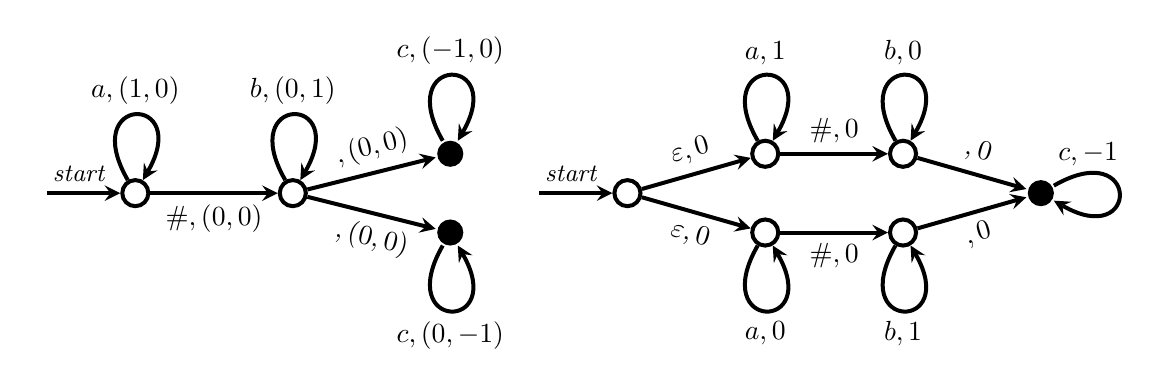
\begin{tikzpicture}
    %===== 2-DVASS =====
    \node (sd) at (-5.75, 0) {};
    \node[draw, circle, minimum size = 0.1in, line width = 0.02in] (ad) at (-4.5,0) {};
    \node[draw, circle, minimum size = 0.1in, line width = 0.02in] (bd) at (-2.5, 0) {};
    \node[fill, circle, minimum size = 0.1in, line width = 0.02in] (c1d) at (-0.5, 0.5) {};
    \node[fill, circle, minimum size = 0.1in, line width = 0.02in] (c2d) at (-0.5, -0.5) {};
    
    \draw[-stealth, line width = 0.02in] (sd) -- node[above, pos = 0.45] {\small\textit{start}} (ad);
    \draw[-stealth, line width = 0.02in] (ad) -- node[below] {$\#, (0, 0)$} (bd);
    \draw[-stealth, line width = 0.02in] (bd) -- node[above, sloped, pos=0.55] {$\eur, (0, 0)$} (c1d);
    \draw[-stealth, line width = 0.02in] (bd) -- node[below, sloped, pos=0.55] {$\gbp, (0, 0)$} (c2d);
    \draw[-stealth, line width = 0.02in] (ad) edge[loop above, distance = 0.5in, out=120, in=60] node[above] {$a, (1, 0)$} (ad);
    \draw[-stealth, line width = 0.02in] (bd) edge[loop above, distance = 0.5in, out=120, in=60] node[above] {$b, (0, 1)$} (bd);
    \draw[-stealth, line width = 0.02in] (c1d) edge[loop, distance = 0.5in, out=120, in=60] node[above] {$c, (-1, 0)$} (c1d);
    \draw[-stealth, line width = 0.02in] (c2d) edge[loop, distance = 0.5in, out=240, in=300] node[below] {$c, (0, -1)$} (c2d);

     %===== 1-VASS =====
    \node (s) at (0.5, 0) {};
    \node[draw, circle, minimum size = 0.1in, line width = 0.02in] (p) at (1.75, 0) {};
    \node[draw, circle, minimum size = 0.1in, line width = 0.02in] (a1) at (3.5, 0.5) {};
    \node[draw, circle, minimum size = 0.1in, line width = 0.02in] (a2) at (3.5, -0.5) {};
    \node[draw, circle, minimum size = 0.1in, line width = 0.02in] (b1) at (5.25, 0.5) {};
    \node[draw, circle, minimum size = 0.1in, line width = 0.02in] (b2) at (5.25, -0.5) {};
    \node[fill, circle, minimum size = 0.1in, line width = 0.02in] (c) at (7, 0) {};
    
    \draw[-stealth, line width = 0.02in] (s) -- node[above, pos = 0.45] {\small\textit{start}} (p);
    \draw[-stealth, line width = 0.02in] (p) -- node[above, sloped] {$\varepsilon, 0$} (a1);
    \draw[-stealth, line width = 0.02in] (p) -- node[below, sloped] {$\varepsilon, 0$} (a2);
    \draw[-stealth, line width = 0.02in] (a1) -- node[above] {$\#, 0$} (b1);
    \draw[-stealth, line width = 0.02in] (a2) -- node[below] {$\#, 0$} (b2);
    \draw[-stealth, line width = 0.02in] (b1) -- node[above, sloped] {$\eur, 0$} (c);
    \draw[-stealth, line width = 0.02in] (b2) -- node[below, sloped] {$\gbp, 0$} (c);
    
    \draw[-stealth, line width = 0.02in] (a1) edge[loop, distance = 0.5in, out=120, in=60] node[above] {$a, 1$} (a1);
    \draw[-stealth, line width = 0.02in] (a2) edge[loop, distance = 0.5in, out=240, in=300] node[below] {$a, 0$} (a2);
    \draw[-stealth, line width = 0.02in] (b1) edge[loop, distance = 0.5in, out=120, in=60] node[above] {$b, 0$} (b1);
    \draw[-stealth, line width = 0.02in] (b2) edge[loop, distance = 0.5in, out=240, in=300] node[below] {$b, 1$} (b2);
    \draw[-stealth, line width = 0.02in] (c) edge[loop, distance = 0.5in, out=30, in=330] (c);
    \node at (7.6, 0.5) {$c, -1$};
\end{tikzpicture}